\documentclass[%
    9pt,
    %handout
]{beamer}
\usepackage{graphicx} % For including single page pdfs
\usepackage{tikz}
\usepackage{layouts}

\usepackage{cambridge_lecture}
\hypersetup{colorlinks=false}



\title{Compromise-free Bayesian sparse reconstruction}
\subtitle{Higson, Handley, Hobson, Lasenby (\href{https://arxiv.org/abs/1809.04598}{arxiv:1809.04598})}
\author[Handley] % (optional, for multiple authors)
{Will Handley\\ \small{wh260@cam.ac.uk}}
\institute[University of Cambridge] % (optional)
{%
    
\includegraphics[width=0.2\textwidth]{kicc.png}\\
    Kavli Institute for Cosmology\\
    Cavendish Laboratory (Astrophysics Group) \\
    University of Cambridge
}
\date{March 19\textsuperscript{th} 2019}

\usepackage{calculator}

\newcommand{\cols}[3][0.5]{%
    \SUBTRACT{1.}{#1}{\wdthb}
    \begin{columns}
        \begin{column}{#1\textwidth}
            #2
        \end{column}
        \begin{column}{\wdthb\textwidth}
            #3
        \end{column}
    \end{columns}
}

\newcommand{\figname}{}
\newenvironment{figright}[2][0.5]{%
    \renewcommand{\figname}{#2}
    \SUBTRACT{1.}{#1}{\wdthb}
    \begin{columns}
        \begin{column}{#1\textwidth}
        }{%
        \end{column}
        \begin{column}{\wdthb\textwidth}
            \includegraphics[width=\textwidth]{\figname}
        \end{column}
    \end{columns}
}

\newcommand{\dfigname}{}
\newenvironment{dfigright}[3][0.5]{%
    \renewcommand{\figname}{#2}
    \renewcommand{\dfigname}{#3}
    \SUBTRACT{1.}{#1}{\wdthb}
    \begin{columns}
        \begin{column}{#1\textwidth}
        }{%
        \end{column}
        \begin{column}{\wdthb\textwidth}
            \includegraphics[width=\textwidth]{\figname}
            \includegraphics[width=\textwidth]{\dfigname}
        \end{column}
    \end{columns}
}



\newenvironment{figleft}[2][0.5]{%
    \SUBTRACT{1.}{#1}{\wdthb}
    \begin{columns}
        \begin{column}{#1\textwidth}
            \includegraphics[width=\textwidth]{#2}
        \end{column}
        \begin{column}{\wdthb\textwidth}
        }{%
        \end{column}
    \end{columns}
}

\newenvironment{dfigleft}[3][0.5]{%
    \SUBTRACT{1.}{#1}{\wdthb}
    \begin{columns}
        \begin{column}{#1\textwidth}
            \includegraphics[width=\textwidth]{#2}
            \includegraphics[width=\textwidth]{#3}
        \end{column}
        \begin{column}{\wdthb\textwidth}
        }{%
        \end{column}
    \end{columns}
}


\newcounter{numimages}

\newenvironment{multifig}[1]{%
    \begin{frame}
        \pdfximage{#1}%
        \setcounter{numimages}{\the\pdflastximagepages}
        \addtocounter{numimages}{-1}

        \begin{tikzpicture}[remember picture, overlay]
            \foreach \pagenum in {1,...,\thenumimages} {%
                \node<handout:0|beamer:\pagenum>[anchor=center] at (current page.center) {
                \includegraphics[width=\textwidth,page=\pagenum]{#1}}; 
            }
            \addtocounter{numimages}{1}
            \node<handout:1|beamer:\thenumimages>[anchor=center] at (current page.center) {
            \includegraphics[width=\textwidth,page=\thenumimages]{#1}}; 
        \end{tikzpicture}
    }{%
    \end{frame}
}


\newcommand{\vect}[1]{\mathbf{#1}}
\newcommand{\bg}[1]{\mathbf{#1}}
\newcommand{\red}[1]{\textcolor{cambblue}{#1}}
\newcommand{\blue}[1]{\textcolor{red}{#1}}
\newcommand{\black}[1]{\textcolor{black}{#1}}
\newcommand{\rr}{\Rightarrow}
\newcommand{\arxiv}[1]{\href{https://arxiv.org/abs/#1}{arXiv:#1}}

\begin{document}

\begin{frame}
    \titlepage{}
\end{frame}



%\begin{frame}
%  \frametitle{Mixture Modelling}
%  \begin{itemize}
%      \item Fit $D$ data points $(\mathbf{x}_d, y_d)$ with some function $y=f(\mathbf{x};\theta)$ with free parameters $\theta$.
%  \end{itemize}
%  \includegraphics{./bsr/results_plots/multi_gg_1d_gg_1d_3_True_1_1000_100_5runs.pdf}
%  \begin{itemize}
%      \item Model function $f(\mathbf{x};\theta)$ as a sum of $N$ basis functions $\varphi(x)$ with weights $a_i$ and location/shape parameters $p_i$, so $\theta=(N,\mathbf{a},\
%  \end{itemize}<++>
%\end{frame}

\begin{frame}
    \frametitle{Bayesian inference}
    \begin{itemize}
        \item Bayes theorem for parameter estimation
            \begin{gather}
                \Pr(D|\theta,M) \times \Pr(\theta|M) = \Pr(\theta|D,M) \times \Pr(D|M) \nonumber\\
                    \mathcal{L}\times\pi = \mathcal{P}\times \mathcal{Z} \qquad
                \mathrm{Likelihood}\times \mathrm{Prior} = \mathrm{Posterior}\times \mathrm{Evidence}\nonumber
            \end{gather}
                \vspace{-15pt}
        \item Bayes theorem for model comparison
            \[
                \Pr(M_i|D) = \frac{\Pr(D|M_i)\Pr(M_i)}{\sum_j \Pr(D|M_j)\Pr(M_j)} \equiv \frac{\mathcal{Z}_i\times\Pi_i}{\sum_j \mathcal{Z}_j\Pi_j}
            \]
            \vspace{-10pt}
        \item Model marginalisation
            \[
                \Pr(\alpha|D) = \sum_j \Pr(\alpha|M_j,D) \Pr(M_j|D) \equiv \sum_j \mathcal{P}_j(\alpha) \times \Pi_j
            \]
            \vspace{-5pt}
        \item Bayesian inference depends on parameter and model priors $\pi(\theta|M)$ and $\Pi(M)$, e.g:
            \begin{itemize}
                \item If the prior adjusts the shape of the likelihood
                \item If the prior changes its width
            \end{itemize}
        \item My definition of \red{Bayesianism} vs \red{Frequentism} is whether you consider this prior dependency a \red{feature} or a \red{bug}.
        \item Other important quantities: Shannon information $\mathcal{I}$, Kullback-Leibler divergence $\mathcal{D}$ and Bayesian model dimensionality $d$ 
            \[
                \mathcal{I}(\theta) = \log \frac{\mathcal{P}}{\pi} \qquad
                \mathcal{D} = \int \mathcal{P} \log \frac{\mathcal{P}}{\pi} d\theta \equiv \left\langle \log \frac{P}{\pi}\right\rangle_\mathcal{P} \equiv \left\langle \mathcal{I} \right\rangle_\mathcal{P} \qquad
                \frac{d}{2} = \left\langle (\mathcal{I}-\mathcal{D})^2\right\rangle_\mathcal{P} \hfill
            \] 
            Handley \& Lemos: \arxiv{1902.04029},   \arxiv{1903.06682}
            
    \end{itemize}
\end{frame}

\begin{frame}
    \frametitle{Bayesian approach to sparse regression}
    \begin{itemize}
        \item Fit $D$ data points $(\vect{x}_d,y_d)$ with some function $y=f(\vect{x};\bg{\theta})$ with free parameters $\bg{\theta}$
    \end{itemize}

    \begin{columns}
        \begin{column}{0.25\textwidth}
            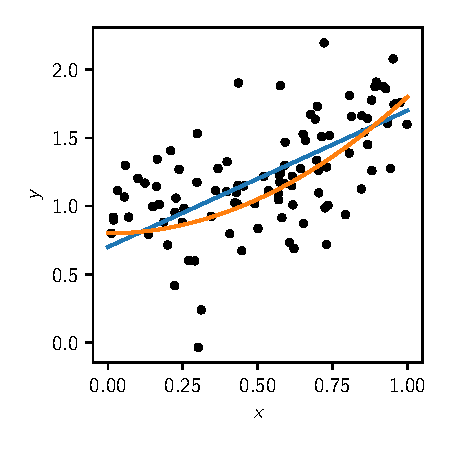
\includegraphics[width=\textwidth]{figures/data_points.pdf}
        \end{column}
        \begin{column}{0.25\textwidth}
            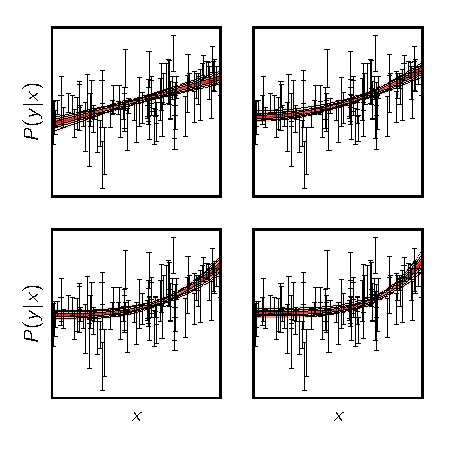
\includegraphics[width=\textwidth]{figures/fgivenx.pdf}
        \end{column}
        \begin{column}{0.5\textwidth}
            \begin{itemize}
                \item If $\vect{x}$ is \red{2-dimensional} 
                    $\rr$ \red{image reconstruction}, etc.
            \end{itemize}

        \end{column}
    \end{columns}

    \begin{itemize}
        \item Model function $f(\vect{x};\bg{\theta})$ as \red{sum} of $N$
            \red{basis functions} $\varphi^{(T)}$ of type $T$,
            with \red{weights} $a_i$ and \red{location/shape} parameters $p_i$, 
            so $\bg{\theta} = (T, N, \vect{a}, \vect{p}_1,\ldots,\vect{p}_N)$:
            \[
                f(\vect{x};\bg{\theta}) 
%= f(\vect{x};T, N, \vect{a}, \vect{p}_1,\ldots,\vect{p}_N) 
                =
                \sum_{i=1}^N a_i\varphi^{(T)}(\vect{x};\vect{p}_i)
            \]
        \item Explore (by sampling) posterior with \red{variable (effective) dimensionality}:
            \[
                \Pr(T,N,\vect{a},\{\vect{p}_i\}|\vect{y})
                \propto \underbrace{\Pr(\vect{y}|T,N,\vect{a},\{\vect{p}_i\})}_{\mbox{likelihood}}
                \underbrace{\Pr(\vect{a}|T)\Pr(\{\vect{p}_i\}|T,N)
                \Pr(N|T)\Pr(T)}_{\mbox{prior}}
            \]
        \item Full \red{posterior} of fit $\Pr(\bg{f}|\bg{y}) = {\displaystyle \int \Pr(\bg{f}|\bg{\theta})\,\Pr(\bg{\theta}|\bg{y})\,d\bg{\theta}}$
            \ldots and that's it!
    \end{itemize}




\end{frame}

\begin{frame}
    \frametitle{Desirable properties}

    $\Pr(T,N,\vect{a},\{\vect{p}_i\}|\vect{y})
    \propto \underbrace{\Pr(\vect{y}|T,N,\vect{a},\{\vect{p}_i\})}_{\mbox{likelihood}}
    \underbrace{\Pr(\vect{a}|T)\Pr(\{\vect{p}_i\}|T,N)
    \Pr(N|T)\Pr(T)}_{\mbox{prior}}$

%$\Pr(T,N,\vect{a},\{\vect{p}_i\}|\vect{y})
%\propto \Pr(\vect{y}|T,N,\vect{a},\{\vect{p}_i\})
%\Pr(\vect{a}|T)\Pr(\{\vect{p}_i\}|T,N)
%\Pr(N|T)\Pr(T)$

    \begin{itemize}
        \item  \red{Full posterior} on parameters 
            (rather than simply optimising) $\rr$ quantify \red{uncertainties}

        \item Bayesian approach $\rr$ naturally penalises \red{overcomplex} models 

        \item \red{Sparsity} can be further \red{enforced directly} by
            $\Pr(N)$ and \red{marginalised over}

        \item No \red{regularisation parameter} to be chosen
            (unlike $L_p$-norm regularisation, etc.)

        \item \red{Variable number} of basis functions with \red{variable positions}

        \item Basis functions \red{families/shapes} determined
            (dictionary learning) or \red{marginalised over}


        \item Can impose \red{arbitrary constraints} on reconstruction 
            (not just positivity)

        \item Accommodates \red{any noise type}, e.g. Gaussian,
            Poisson, etc. (extra \red{hyperparameters})


        \item Accommodates arbitrary \red{missing} and/or \red{irregular} data 

    \end{itemize}
\end{frame}

\begin{frame}
    \frametitle{Practical considerations}

    $\Pr(T,N,\vect{a},\{\vect{p}_i\}|\vect{y})
    \propto \underbrace{\Pr(\vect{y}|T,N,\vect{a},\{\vect{p}_i\})}_{\mbox{likelihood}}
    \underbrace{\Pr(\vect{a}|T)\Pr(\{\vect{p}_i\}|T,N)
    \Pr(N|T)\Pr(T)}_{\mbox{prior}}$

    \begin{itemize}
        \item \red{Transdimensional sampling}
            (RJMCMC) costly $\Rightarrow$ use \red{product-space} approach
            \newline -- consider \red{hypermodel} $H$ with space $\bg{\theta}$ of
            \red{fixed dimensionality} $T_{\rm max} \times N_{\rm max}$
            \newline -- integer parameters $(T,N)$ enumerate models $H_M$ within $H$
            \newline -- for each sampled $(T,N)$-values, \red{partition} $\bg{\theta}$ into
            parameters used by $H_M$ and others
            \newline -- latter set of parameters \red{ignored} (not passed by
            `wrapper' to likelihood for $H_M$)

        \item \red{Marginalisation} over $\vect{a}$ and
            $\{\vect{p_i}\}$ $\Rightarrow$ posterior $\Pr(T,N|\vect{y})$ (\red{recovers
            PORs})
            \[
                \red{
                    {\cal P}_{(T,N)}^{(T',N')} = \ln\left[\frac{\Pr(T',N'|\vect{y})}{\Pr(T,N|\vect{y})}\right]
                }
            \]
        \item
            i.e.\ Bayesian model selection 
            \red{without evidences!} (can also use \red{`vanilla'} method)

        \item \blue{But\ldots} 
            \newline -- posterior $\Pr(T,N,\vect{a},\{\vect{p}_i\}|\vect{y})$ 
            dimensionality $N_{\rm dim} \sim 10^3-10^4$ for \red{small images} 
            \newline -- posterior is \red{highly multimodal} with \red{strong degeneracies}
            (certainly non-convex!)
            \newline -- \red{categorical/integer} parameters $T,N$ $\Rightarrow$ cannot use
            \red{gradients}


            $\blue{\Rightarrow}$ use \blue{(dynamic) nested sampling} to explore posterior
            with \red{(dy)PolyChord}

        \item Computationally \red{demanding}, but now
            \red{possible} (proof of principle) \ldots 
    \end{itemize}

\end{frame}

% Possible slide on nested sampling
\begin{frame}
    \frametitle{Nested sampling}
    \begin{itemize}
        \item Want to compute evidence, which is high-dimensional integral over parameter space $\theta$. Define prior volume $X$ as fraction of prior above contour $\mathcal{L}(\theta)\ge \mathcal{L}$
            \[\mathcal{Z} = \int \mathcal{L}(\theta) \pi(\theta) d\theta = \int \mathcal{L}(X) dX, \qquad X(\mathcal{L}) = \int_{\mathcal{L}(\theta)\ge\mathcal{L}} \pi(\theta) d\theta \]
        \item Nested sampling procedure:
            \begin{enumerate}
                \item Draw $N$ ``live'' points from the prior $\pi(\theta)$ and compute likelihoods.
                \item Remove lowest live point, replace with one drawn from prior at higher likelihood.\label{step2}
                \item Repeat step \ref{step2} until live points occupy a small enough prior volume.
            \end{enumerate}
        \item Procedure allows one to estimate prior volumes probabilistically, as volume contracts by factor $\approx\frac{N}{N+1}$ at each step.
        \item Compute evidence from $M$ discarded points via trapezium rule:
            \[ \mathcal{Z} \approx \sum_{i=0}^{M} \mathcal{L}_i \times \frac{1}{2}(X_{i-1}-X_{i+1}), \qquad X_0=1, \quad X_N =0, \quad X_i= t_i X_{i-1}, \quad \Pr(t_i) = N t^{N-1}  \]
        \item Generates posteriors as by-product with weights $w_i = \frac{1}{\mathcal{Z}}\mathcal{L}_i \times \frac{1}{2}(X_{i-1}-X_{i+1})$
        \item Step \ref{step2} is by far the hardest step.
            \begin{description}
                \item[MultiNest] Ellipsoidal based rejection sampling
                \item[Galilean] Gradient-based HMC-like algorithm
                \item[Diffusive NS \& Dynesty] User-based choice
                \item[PolyChord] Slice-sampling 
            \end{description}

    \end{itemize}

\end{frame}

\begin{frame}
    \frametitle{Simple basis functions}

    \begin{itemize}
        \item 1-d generalised Gaussians $\varphi^{\rm (g)}(x;\bg{p}) = \varphi^{\rm (g)}(x;\mu,\sigma,\beta) = e^{-(|x-\mu|/\sigma)^\beta}$ (GGMM)
        \item 1-d tanh functions  $\varphi^{\rm (t)}(x;\bg{p}) = \varphi^{\rm (t)}(x;w,b) = \tanh(wx+b)$ (TMM)
            \vfill
            \includegraphics[width=0.49\textwidth]{BSR/diagrams/gg_demo}\hfill
            \includegraphics[width=0.49\textwidth]{BSR/diagrams/ta_demo}
        \item Easily extended to \red{higher dimensions} (including
            \red{anisotropic scaling} and \red{rotation})
    \end{itemize}
\end{frame}

\begin{frame}
    \frametitle{Simple 1-D examples: generalised Gaussians data}

    \includegraphics[width=0.59\textwidth]{BSR/results_plots/multi_gg_1d_gg_1d_2_True_1_1000_100_5runs}\hfill
    \includegraphics[width=0.35\textwidth]{BSR/results_plots/odds_gg_1d_gg_1d_2_5runs}
    \includegraphics[width=0.59\textwidth]{BSR/results_plots/multi_gg_1d_gg_1d_3_True_1_1000_100_5runs}\hfill
    \includegraphics[width=0.35\textwidth]{BSR/results_plots/odds_gg_1d_gg_1d_3_5runs}
    \includegraphics[width=0.59\textwidth]{BSR/results_plots/multi_adfam_gg_ta_1d_gg_1d_1_True_1_1000_100_5runs}\hfill
    \includegraphics[width=0.35\textwidth]{BSR/results_plots/odds_adfam_gg_ta_1d_gg_1d_1_5runs}
\end{frame}

\begin{frame}
    \frametitle{Simple 2-D examples: generalised Gaussians data}

\includegraphics[width=0.59\textwidth]{BSR/results_plots/multi_gg_2d_gg_2d_1_True_1_2000_250_5runs.pdf}\hfill
\includegraphics[width=0.35\textwidth]{BSR/results_plots/odds_gg_2d_gg_2d_1_5runs.pdf}
\includegraphics[width=0.59\textwidth]{BSR/results_plots/multi_gg_2d_gg_2d_2_True_1_2000_250_5runs.pdf}\hfill
\includegraphics[width=0.35\textwidth]{BSR/results_plots/odds_gg_2d_gg_2d_2_5runs.pdf}
\includegraphics[width=0.59\textwidth]{BSR/results_plots/multi_gg_2d_gg_2d_3_True_1_2000_250_5runs.pdf}\hfill
\includegraphics[width=0.35\textwidth]{BSR/results_plots/odds_gg_2d_gg_2d_3_5runs.pdf}
\end{frame}

\begin{frame}
    \frametitle{HST eXtreme Deep Field images: generalised Gaussians fit}

\includegraphics[width=0.59\textwidth]{BSR/results_plots/multi_gg_2d_get_image_1_True_1_2000_250_5runs.pdf}\quad 
\includegraphics[width=0.35\textwidth]{BSR/results_plots/odds_gg_2d_get_image_1_5runs.pdf}                       
\includegraphics[width=0.59\textwidth]{BSR/results_plots/multi_gg_2d_get_image_2_True_1_2000_250_5runs.pdf}\quad 
\includegraphics[width=0.35\textwidth]{BSR/results_plots/odds_gg_2d_get_image_2_5runs.pdf}                       
\includegraphics[width=0.59\textwidth]{BSR/results_plots/multi_gg_2d_get_image_3_True_1_2000_250_5runs.pdf}\quad 
\includegraphics[width=0.35\textwidth]{BSR/results_plots/odds_gg_2d_get_image_3_5runs.pdf}                       
\end{frame}

\begin{frame}
\frametitle{Bayesian neural networks}

\begin{itemize}
\item Consider \red{feed-forward NN}, $d$-dimensional input $\vect{x}$, one hidden layer with $N$ nodes:\\[0.4cm]
%
\begin{columns}
	\begin{column}{0.4\textwidth}
		\includegraphics[width=\textwidth]{BSR/diagrams/nn_diagram}
	\end{column}
\begin{column}{0.6\textwidth}
\begin{eqnarray*}
a^{[1]}_j & = & \phi^{[1]}\left(\sum_{i=1}^d x_i w^{[1]}_{ji} +
b_j^{[1]}\right)\\
\hat{y}_j = a^{[2]}_j & = & \phi^{[2]}\left(\sum_{i=1}^N a_i^{[1]}w^{[2]}_{ji} + b_j^{[2]}\right)
\end{eqnarray*}
\end{column}
\end{columns}

\item If activation functions $\phi^{[1]}(x)=\tanh x$ and $\phi^{[2]}(x)=x$, and $b_j^{[2]}=0$
\newline $\Rightarrow$ consider (noisy) \red{data points} 
$(\vect{x}^{(t)},y^{(t)})$ $(t=1,2,\ldots,T)$ as training set
\newline\phantom{$\rr$} 
with \red{objective function} equal to \red{likelihood}
$\Pr(\bg{y}|\hat{\bg{y}})$ (noise model)\\[0.2cm]
%from $d$-dimensional function $f(\vect{x})$ (with noise on output)
%\newline 
$\Rightarrow$ \red{regression problem} with $N$ 
adaptive \red{tanh basis functions} (or
$\mbox{sig}(x)$ or $\mbox{max}(0,x)$)
%
\[
\red{
\hat{y}(\vect{x}) = f(\vect{x}) = \sum_{j=1}^N a^{[1]}_j \tanh
\left(\sum_{i=1}^d x_iw^{[1]}_{ji} +
b_j^{[1]}\right)\qquad\black{\mbox{(Activation function MM)}}
}
\]
%
\end{itemize}

\end{frame}

\begin{frame}
\frametitle{Bayesian neural networks architecture}

\begin{itemize}

\item \red{In general}: NN can have $L$ \red{hidden layers} with
\red{nodes} $N^{[1]},\ldots,N^{[L]}$ \& many \red{outputs}
\item output(s) no longer \red{direct sum(s)} of inputs but \red{method
still applicable}
\item can \red{determine integer parameters}
$(L,\{N^{[l]}\})$ and \red{activation type} $T$
\item \red{simultaneous} training of network \red{parameters},
\red{architecture} and \red{activation function}
\item \red{full joint posterior} distribution on \red{all
aspects} of NN

\end{itemize}

\end{frame}

\begin{frame}
    \frametitle{2-D examples: generalised Gaussians \& HST images}

\includegraphics[width=0.59\textwidth]{BSR/results_plots/multi_nn_2l_get_image_3_True_1_2000_250_5runs.pdf}\qquad 
\includegraphics[width=0.35\textwidth]{BSR/results_plots/odds_nn_2l_get_image_3_5runs.pdf}                        
\includegraphics[width=0.59\textwidth]{BSR/results_plots/multi_nn_2l_get_image_2_True_1_2000_250_5runs.pdf}\qquad 
\includegraphics[width=0.35\textwidth]{BSR/results_plots/odds_nn_2l_get_image_2_5runs.pdf}                        
\includegraphics[width=0.59\textwidth]{BSR/results_plots/multi_nn_adl_gg_2d_3_True_1_2000_250_5runs.pdf} 
\includegraphics[width=0.35\textwidth]{BSR/results_plots/odds_nn_adl_gg_2d_3_5runs.pdf} 
\end{frame}

\begin{frame}
    \frametitle{Bayesian inference from simulations}
    \framesubtitle{(a.k.a. Likelihood Free Inference)}

    \begin{itemize}
        \item In many cases, do not have access to likelihood $\Pr(D|\theta,M)$
        \item Can however simulate data $D=\phi(\theta,M)$
        \item Must compress data in order to avoid curse of dimensionality $t = t(D)$
        \item Massive compression: $\mathrm{dim}(t)=\mathrm{dim}(\theta)$ (Alsing et al \arxiv{1801.01497})
    \end{itemize}
    \begin{enumerate}
        \item Construct proxy joint/conditional distribution $p=\Pr(t,\theta|\eta)$ with nuisance $\eta$:
            \begin{itemize}
                \item Gaussian mixture model, $x=(t,\theta)$, $\eta = (N, A_1,\mu_1,\sigma_1,\ldots,A_N,\mu_N, \sigma_N)$: 
                    \[p(t,\theta|\eta) = \sum_{i=1}^N A_i\exp\left(-\frac{(x-\mu_i)^2}{2\sigma_i^2}\right) \quad \text{\black{(Alsing et al \arxiv{1801.01497})}}\]
                    \vspace{-5pt}
                \item Neural density estimator $x=(t,\theta)$, $\eta = (\mathrm{Architecture}, \mathbf{w})$ \\(Alsing et al \arxiv{1903.00007}): 
            \end{itemize}
        \item Compute example simulations $\{(t_i, \theta_i)\}$
        \item Fit proxy to simulations via $\eta$ given prior $\Pr(\eta)$, using likelihood
            \[\mathcal{L}(\eta) = \prod_i p(t_i,\theta_i|\eta) \]
            \vspace{-10pt}
        \item Marginalise over proxy (ignore $\eta$ column in samples), evaluated at observed data $D$
            \[\Pr(\theta,D) = \int p(\theta,t(D)|\eta)\Pr(\eta) d\eta \]
            \vspace{-10pt}
        \item Condition on data $D$, either analytically or via nested sampling
            \vspace{-3pt}
            \[\Pr(\theta|D) = \Pr(\theta,D)/\Pr(D) \qquad \Pr(D) = \int \Pr(\theta,D) d\theta\]
    \end{enumerate}
\end{frame}

\begin{frame}
    \frametitle{Likelihood free inference: what's in a name?}
    \begin{itemize}
        \item The term ``Likelihood-free'' is a misnomer -- there is still very much a likelihood involved at the centre of the analysis, we just don't analytically compute it
        \item From the Bayesian viewpoint, in lieu of attempting an impossible calculation of a likelihood, we construct a proxy, and marginalise over our lack of knowledge.
        \item Before becoming involved in this hack week, I found the term LFI disconcerting.
        \item Alternative names
            \begin{itemize}
                \item Simulation-based inference
                \item Likelihood learning
            \end{itemize}
        \item Proposed Hack: Come up with a different name for those outside the field
    \end{itemize}
\end{frame}


\end{document}
